% !TEX root =main.tex
We illustrate our technique on a two-dimensional switched system with $4$ modes. We fix the confidence level, \mbox{$\beta = 0.92$}, and compute the lower and upper bounds on the JSR for $N:=15+15k,\, k \in\{0, \ldots, 23\}$, according to Theorem~\ref{thm:lowerbound} and Theorem~\ref{thm:mainTheorem}, respectively. We illustrate the average performance of our algorithm over $10$ different runs in Fig.~ \ref{fig:11} and Fig.~\ref{fig:21}. Fig.~\ref{fig:11} shows the evolution of $\delta(\beta, N)$ as $N$ increases. We illustrate that $\delta$ converges to $1$ as expected. In Fig.~\ref{fig:21}, we plot the upper bound and lower bound for the JSR of the system computed by Theorem~\ref{thm:mainTheorem} and Theorem~\ref{thm:lowerbound}, respectively. To demonstrate the performance of our technique, we also provide the JSR approximated by the JSR toolbox \cite{jsrtoolbox}, which turns out to be $0.7727$. Note that, the plot for the upper bound starts from $N=45$. This is due to the fact for $N=15$, and $N=30$, $\delta(\beta, \omega_N) = 0$, hence it is not possible to compute a nontrivial upper bound for these small values of $N$. As can be seen, the upper bound approaches to a close vicinity of the real JSR with approximately 200 samples. In addition, the gap between the upper and lower bound converges to a multiplicative factor of $\frac{\rho}{\sqrt{n}}$ as expected.

\begin{figure}
\begin{center}
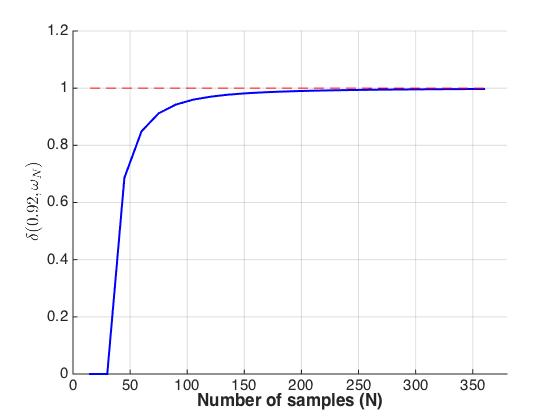
\includegraphics[trim = 5mm 5mm 5mm 5mm, scale=0.35]{delta1.jpg}

\caption{Evolution of $\delta$ with increasing $N$.}
\label{fig:11}
\end{center}
\end{figure}

\begin{figure}
\begin{center}
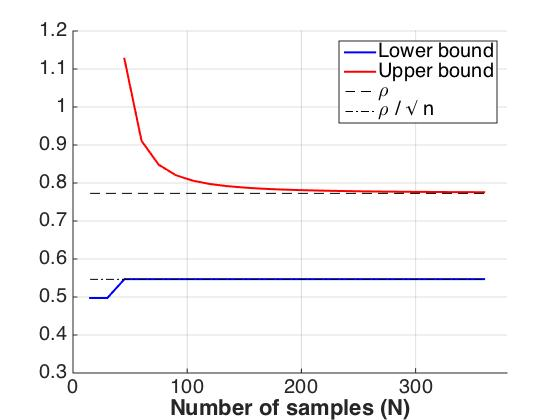
\includegraphics[trim = 5mm 5mm 5mm 5mm,scale=0.35]{bounds1.jpg}

\caption{Evolution of the upper and lower bounds on the JSR with increasing $N$, for $\beta=0.92$.}
\label{fig:21}
\end{center}
\end{figure}

Note that, if we increase the dimension of the switched system, the convergence of $\delta$ to $1$ will become much slower. We confirmed this via experiments up to dimension $n=6$. For example, for dimension $n=4$, it took $N=5,000$ to $N=10,000$ points to reach $\delta = 0.9$. We nevertheless observe convergence of the upper bound to $\rho(\calM)$, and convergence of the lower bound to $\frac{\rho(\calM)}{\sqrt{n}}$. The gap between these two limits is $\frac{\rho}{\sqrt{n}}$ and could be improved by considering a more general class of common Lyapunov functions, such as those that can be described by sum-of-squares polynomials \cite{sosLyap}. We leave this for future work.

Finally, we randomly generate $10,000$ test cases with systems of dimension between $2$ and $7$, number of modes between $2$ and $5$, and size of samples $N$ between $30$ and $800$. We take $\beta = 0.92$ and we check if the upper bound computed by our technique is greater than the actual JSR of the system. We get $9873$ positive tests, out of $10,000$, which gives us a probability of $0.9873$ of the correctness of the upper bound computed. Note that, this probability is significantly above the provided $\beta$. This is expected, since our techniques are based on worst-case analysis and thus fairly conservative.

\begin{subsection}{Networked Control System}\label{networkedEx}
We now consider a linear time-invariant control system given as \mbox{$x_{k+1}=Ax_k+Bu_k$,} where we do not have access to its dynamics given by the matrices $A$ and $B$. The control law is of the form $u_k = Kx_k$, where $K$ is also unknown. The open-loop system is unstable with eigenvalues at $\{0.45, 1.1\}$. The controller stabilizes the system by bringing its eigenvalues to $\{0.8, -0.7\}$.
%\begin{equation*}A = \begin{bmatrix} 1.14 &0.365 \\ 0.82 &1.95\end{bmatrix}, B = \begin{bmatrix} 0.5 \\ 0.2 \end{bmatrix}.
%\end{equation*}
%The control law is of the form $u_k = Kx_k$, where \mbox{$K = \begin{bmatrix} 0.9 & 0.75 \end{bmatrix}$}.
The control input is transmitted
over a wireless communication channel that is utilized by $\ell$ users, including the controller. The communication between the users and the recipients is performed based on the IEEE 802.15.4 MAC layer protocol \cite{macLayer}, which is used in
some of the proposed standards for control over wireless, e.g., WirelessHART \cite{wirelessHart}. This MAC layer integrates both guaranteed slots and contention based slots. In this example, we consider a beacon-enabled mode of the MAC protocol. In this setup, a centralized control user periodically synchronizes and configures all the users. This period is named Beacon Interval. This interval is divided into two intervals: active and inactive period. The active period is divided into 6 slots. The first 2 slots correspond to the contention access period (CAP), and the next 4 slots correspond to the collusion free period (CFP). In the CAP, the users can only send their message if the channel is ``idle'' with carrier-sense multiple access with collision avoidance (CSMA/CA). In the CFP however, each user has guaranteed time slots, during which there are no packet losses. In our example, the third and fourth slots are designated for the controller, while the fifth and sixth slots are allocated to the other users. Finally, during the inactive period, all users enter a low-power mode to save energy. We illustrate the overall structure of this communication protocol in Fig.~\ref{comExample}. 
We now want to decide whether the resulting closed-loop network control system is stable by simulating it starting from different initial conditions. 
\begin{figure}
\begin{center}
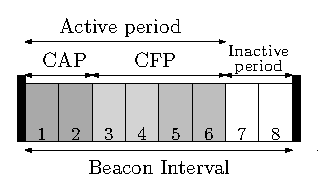
\includegraphics[scale= 1.5]{comNetwork.eps}
\end{center}
\caption{The time allocation structure of the modified IEEE 802.15.4 MAC layer.}
\label{comExample}
\end{figure}

Note that, the closed-loop dynamics of the underlying system when the controller is active is $A_c = A+BK$. Then, we can model the overall networked control system by the linear switched system $x_{k+1} = \bar{A}x_k$, where $\bar{A} \in \calM$ and
\begin{equation}\label{eqn:calCom}\calM = \{A^2A_c^2A^4, A_cAA_c^2A^4,AA_c^3A^4, A_c^4A^4\}.
\end{equation}
Note that, in \eqref{eqn:calCom}, each mode corresponds to a different utilization of the CFP by the users. For example, the mode defined by $A_cAA_c^2A^4$ is active when the first slot in the CFP is assigned to the controller and the second slot is assigned to the other users. We assume that all of the users using the channel have an equal probability of being assigned to a time slot during the CFP. Therefore, the probability of each mode in $\calM$ being active is $\left\{\frac{1}{(\ell-1)^2}, \frac{1}{\ell(\ell-1)}, \frac{1}{(\ell-1)\ell}, \frac{1}{\ell^2}\right\}$, i.e., the modes given in \eqref{eqn:calCom} will not be active with the same probability. Hence, we make use of Remark \ref{rem:probGeneralize} and update our bounds accordingly. Fig.~\ref{fig:4} shows the computed bounds. As can be seen, approximately after 500 samples,  the upper bound on the JSR drops below $1$, which lets us decide that the given closed-loop networked control system is stable, with probability $0.95$.

\begin{figure}
    \centering
        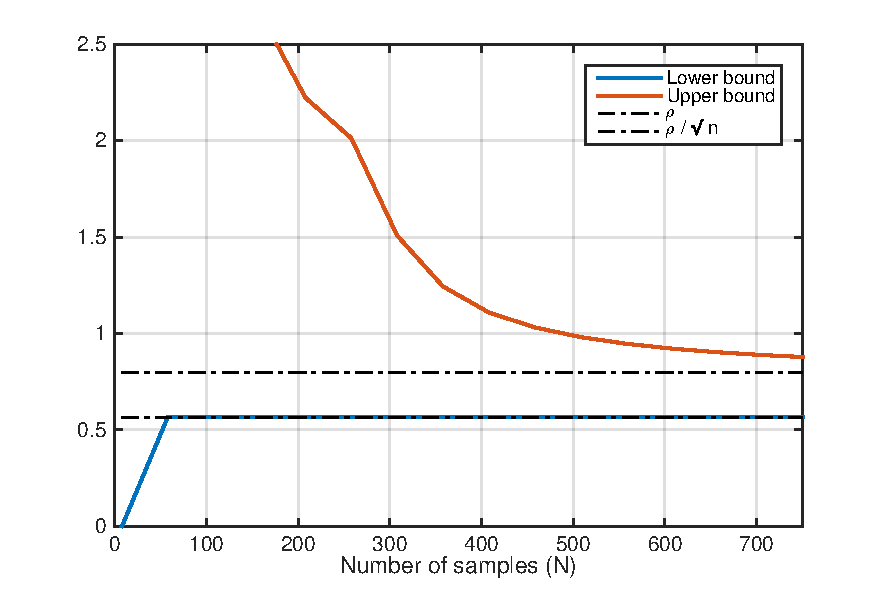
\includegraphics[scale=0.7]{networkControl.pdf}
    \caption{The evolution of the computed upper and lower bounds on the JSR with respect to the number of simulations collected from the networked control system.}
        \label{fig:4}
\end{figure}

\end{subsection}